\chapter{Background}
\label{chap:background}


\section{Overview}
\label{sec:overview}

During the last 15 years, there has been an increasing number of publications which harmonically combine the \textit{Software Engineering} field with that of \textit{Data Mining}. The combination of these two fields has led to the generation of a new research area, that of \textit{Mining Software Repositories} (MSR). More interestingly, an international workshop on MSR\footnote{\url{http://msrconf.org}} has been organised as part of the \textit{International Conference on Software Engineering}\footnote{\url{http://www.icse-conferences.org/}} (ICSE), since 2004. The organisers of this workshop consider the MSR field as the one that ``analyses the rich data available in software repositories to uncover interesting and actionable information about software systems and projects.''


\section{Mining Software Repositories}
\label{sec:msr}

Since the official birth of the MSR field, in 2004, there have been a few publications that aim to provide an overview of this field. \nolink{\citeauthor{Hassan:2008}} \cite{Hassan:2008} identifies historical repositories, such as source-control\footnote{Commonly known as \textit{version} or even \textit{revision control} repositories. Popular examples include \textit{Git} (with \textit{GitHub} being the most prevalent service of this type), and \textit{Subversion} controls.} and bug repositories, as the main type of software repositories, to be mined for revealing interesting information about software projects.

Regarding the methodology used for the purposes of MSR, \nolink{\citeauthor{Kagdi:2007}} mention, among others, the static source code analysis, which is used extensively for bug finding and fixing, or even Information Retrieval methods, which are used for classification and clustering of similar documents. They also discuss frequent pattern mining, with the purpose of mining usage patterns, referring to the popular \textit{Dynamine} system, presented in \cite{Livshits:2005}. This has been one of the first systems to mine usage patterns, with its key hypothesis being that ``violations of useful patterns are potential sources of errors''. 

After an overview of surveys such as the one conducted by \nolink{\citeauthor{Kagdi:2007}}, we see that the early systems in the MSR field mainly targeted bug identification. Although this purpose is still popular, the large amount of source code that is now available in software repositories, as well as the increasing trend in leveraging third party libraries, that aim to facilitate the coding process, introduced a new aspect for mining software repositories; that of mining usage patterns that target the APIs of popular third-party libraries.


\section{Mining API Usage Patterns}
\label{sec:api-usage}

%On top of the aforementioned analysis, the fact that a large amount of queries on the web for the Java language are related to APIs, as well as %that most of the latter lack any sufficient explanation, as mentioned in \Cref{chap:introduction}, has prompted many researchers to mine %software repositories with the purpose of extracting API usage examples. 

Indeed, \nolink{\citeauthor{Khatoon:2011}} \cite{Khatoon:2011} identify \textit{API usage} as one of the three primary source code mining scopes\footnote{With \textit{programming rules} and \textit{copy-paste detection} being the other two.}. \nolink{\citeauthor{Ishag:2016}} \cite{Ishag:2016} define the problem of API usage pattern mining as ``the process of finding the proper usage sequence or order of a group of reusable code elements within an API''. This requires searching for API source code inside client code -located in local software repositories or in the web- which, at a method level, may be reduced to API methods (referred to as \textit{API method calls} or even as \textit{method calls}), inside \textit{client methods}, as these are defined below:

\begin{description}
\item[Client code] A source code file, that may contain usages of the target API.
\item[Client method] A method of the client code.
\item[API method call] A method of the API that is invoked inside a client method.
\end{description}

The first step in order for a collection of source code files to be mined for existing -frequent- patterns, is to determine on the preprocessing approach of the available source code. According to \nolink{\citeauthor{Ishag:2016}} \cite{Ishag:2016} there are three paths of mining techniques based on the way the datasets are preprocessed; namely \textit{itemsets}, \textit{sequences} and \textit{graphs}.

In this section we are going to explain both of them. For the sake of a better understanding of the differences between these three paths of minings techniques, we firstly provide a list of indicative snippets, in \Cref{fig:client-method-examples}.

\begin{figure}[t]
  \begin{subfigure}[b]{0.3\textwidth}
    \lstinputlisting{listings/Example1.java}
    \caption{}
    \label{listings:example1}
  \end{subfigure}
  \begin{subfigure}[b]{0.3\textwidth}
    \lstinputlisting{listings/Example2.java}
    \caption{}
    \label{listings:example2}
  \end{subfigure}
  \begin{subfigure}[b]{0.3\textwidth}
    \lstinputlisting{listings/Example3.java}
    \caption{}
    \label{listings:example3}
  \end{subfigure}
  \caption[Examples of API method calls inside client code]{Client method examples where the API methods are called (\subref{listings:example1}) once in a fixed order, (\subref{listings:example2}) more than once in a fixed order, and (\subref{listings:example3}) more than once in a random order.}
\label{fig:client-method-examples}
\end{figure}


\subsection{Itemset Mining}
\label{subsec:itemset-mining}

Generally speaking, an \textit{itemset} is a collection of unique items, where the order in which the items show is not preserved. The most popular use of this representation is linked to the \textit{market-basket analysis\footnote{\url{http://snowplowanalytics.com/guides/recipes/catalog-analytics/market-basket-analysis-identifying-products-that-sell-well-together.html}}}, which describes many-to-many relationships between baskets (also called \textit{transactions}, and defined in \Cref{def:transaction}) and itemsets \cite{Rajaraman:2012}. For instance, a basket may relate to the itemset $\{cheese$, $bacon$, $bread\}$.

\begin{defn}
\label{def:transaction}
Using a set of items $I=\{i_1,i_2,...,i_n\}$, a transaction $T$ can be represented as a tuple in the form ($id$, $items$), where $id$ uniquely identifies $T$, while $items$ indicates a subset of items in $I$.
\end{defn}

Itemset mining is then linked to \textit{association rule mining}, where an association rule indicates a frequent relation in the form $\{cheese$,$bacon\}$ $\rightarrow$ $\{bread\}$, which means that a client that buys the set of items on the left hand would probably also buy the set of items on the right hand. In addition to the market basket data domain, this concept has been applied to a large number of other domains, including Web mining, bioinformatics, and medical diagnosis \cite{Tan:2005}. 

In terms of source code and more specifically of method calls, we can think of a client method as a transaction, and of the API method calls in it as its itemset. Table \ref{tab:itemset-example} shows the transactions generated when the API method calls of the client methods presented in \Cref{fig:client-method-examples} are represented as itemsets. As we can see, every transaction consists of a ``bag'' of API calls, thus omitting any information about multiple invocations of the same API method, and about the order on which the API methods are called.

\begin{table}[ht]
\centering
\small
\caption[Representing the API method calls as an itemset]{Transactions generated when the API method calls presented in \Cref{fig:client-method-examples} are represented as itemsets.}
\label{tab:itemset-example}
\begin{tabular}{ll}
\toprule
\textsf{Transaction} & \textsf{Itemset}\\
\midrule
%
\textsf{$client\_m_1$} & \textsf{$\{API\_m_1$, $API\_m_2$, $API\_m_3\}$} \\
%
\textsf{$client\_m_2$} & \textsf{$\{API\_m_1$, $API\_m_2$, $API\_m_3\}$} \\
\textsf{$client\_m_3$} & \textsf{$\{API\_m1$, $API\_m_2$, $API\_m_3\}$} \\
\bottomrule
\end{tabular}
\end{table}

A large number of general-purpose algorithms that mine itemsets have been proposed, including the popular \textit{Apriori} \cite{Agrawal:1994} or the \textit{FP-growth} \cite{Han:2000} algorithms, while there are several publications on mining frequent (or interesting) itemsets that target source code, aiming to facilitate API usage \cite{Li:2005, Livshits:2005}\cite{Fowkes:2015}. The definition of a frequent itemset is given in \Cref{def:freq-itemset}.

\begin{defn}
\label{def:freq-itemset}
Given a support threshold $min\_sup$, an itemset $I$ with support $sup(I)$ is a frequent one, if $sup(I)\geq min\_sup$. The support of an itemset indicates the number of transactions that contain the itemset.
\end{defn}

Note that, although the \textit{interestingness} of an itemset/sequence had at first been linked to its frequency in a given database, most recent approaches use statistical models to mine interesting itemsets/sequences.


\subsection{Sequence Mining}
\label{subsec:sequence-mining}

Similarly to an itemset, a \textit{sequence} is a collection of items, however, in this collection, the order in which the items show is preserved, while duplicates may exist.

Table \ref{tab:sequence-example} shows the transactions generated when the API method calls of the client methods presented in \Cref{fig:client-method-examples} are represented as sequences.

\begin{table}[ht]
\centering
\small
\caption[Representing the API method calls as a sequence]{Transactions generated when the API method calls presented in \Cref{fig:client-method-examples} are represented as sequences.}
\label{tab:sequence-example}
\begin{tabular}{ll}
\toprule
\textsf{Transaction} & \textsf{Sequence}\\
\midrule
%
\textsf{$client\_m_1$} & \textsf{$\{API\_m_1$, $API\_m_2$, $API\_m_3\}$}\\
%
\textsf{$client\_m_2$} & \textsf{$\{API\_m_1$, $API\_m_1$, $API\_m_2$, $API\_m_3\}$}\\
\textsf{$client\_m_3$} & \textsf{$\{API\_m_2$, $API\_m_3$, $API\_m_1$, $API\_m_2\}$}\\
\bottomrule
\end{tabular}
\end{table}

Sequence mining is a well studied problem; there is a great research in mining DNA sequences, or even time-series, while there are numerous algorithms that perform sequence mining. Some striking examples include the \textit{SPADE} algorithm \cite{Zaki:2001} that mines frequent sequences (defined in \Cref{def:freq-sequence}), and the \textit{BIDE} algorithm \cite{Wang:2004} which is used extensively in systems that conduct API usage mining in order to mine frequent closed sequences (defined in \Cref{def:freq-closed-sequence}). Moreover, algorithms that mine interesting sequences rather than frequent ones have emerged during the last years \cite{Fowkes:2016}.

\begin{defn}
\label{def:freq-sequence}
Similarly to a frequent itemset, a sequence $S$ with support $sup(S)$ is frequent if, given a support threshold $min\_sup$, it holds that $sup(S)\geq min\_sup$.
\end{defn}

\begin{defn}
\label{def:freq-closed-sequence}
A \textit{frequent closed sequence} is a frequent sequence for which there is no super-sequence with the same support.
\end{defn}


\subsection{Graph Mining}
\label{subsec:graph-mining}

The most common way to represent a source code file is using an \textit{Abstract Syntax Tree} (AST), which provides a convenient way to preserve useful nodes, while excluding others (e.g. parentheses, semicolons, etc.). An AST is an intermediate tree representation of the source code, and is the result of the reduction of a \textit{parse tree}, produced by a parser generator. The concept behind this reduction is that a parse tree usually contains numerous nodes, most of which are furthermore redundant, in the sense that they do not contain any structure information. An indicative example of the AST representation used in the current project is presented in \Cref{sec:srcml-example}, where we also illustrate the AST for a given source code, in \Cref{listings:srcml-ast}.

ASTs tend to be a simpler source code representation structure than the \textit{Abstract Semantic Graphs} (ASG), which provide a higher level of abstraction than the first ones, and that are typically constructed from an AST by a process of enrichment and abstraction.

Interestingly, the first step in order to mine source code  in -almost- any case is to extract an AST for each of the source code files. Taking this into account, one could take advantage of as much information as possible stored in these trees. That is, although itemset and sequence mining have been proven efficient in terms of computational complexity, both of these representations lead to loss of information when they are used to represent structured text, such as source code.

In general, a more efficient way in that case would be to use a directed graph, where nodes represent statements in the source code, and edges indicate possible transitions between the statements. Common graph-based structures used in source code mining include \textit{Control Flow Graphs} (CFGs), which tend to represent the paths that might be traversed through a program during its execution, or even the \textit{Program Dependency Graphs} (PDGs), that capture dependencies between statements.

However, this huge quantity of information comes with a great computational cost. Indeed, working with CFGs and PDGs may seem an infeasible solution when mining large repositories.

Regarding API usage mining, the API method calls of a client code could be well represented either by a tree structure, as shown in \Cref{listings:graph-tree}, where the representation mainly captures the different levels on which the API methods are invoked, or even by a simplified graph, as the one illustrated in \Cref{listings:graph-graph}, which depicts a sequence of API calls, preserving loop and condition statements.

There has been a large number of frequent subgraph algorithms implemented so far \cite{Yan:2002, Huan:2004}. However, in the field of API mining, frequent subtree mining seems to be more common, and thus frequent subtree mining algorithms are usually applied to solve the problem of mining API usage patterns, with the data being represented using a tree structure.

With the purpose of leveraging a frequent subtree algorithm, one has to generate a database of transactions, similarly to the itemset mining problem. This can be achieved quite easily by serialising the tree using a delimiter, and a character that indicates level change. 

For instance, the tree illustrated in \ref{listings:graph-tree} can be well transformed to the transaction below:
\begin{align*}
\{m_1,m_2,m_3,-1,m_4,-1,-1,-1\}
\end{align*}

\noindent
where the comma (``,'') character is used as the delimiter between the API methods, and the number $-1$ indicates a level-up move\footnote{A careful reader may observe that such a transaction is quite similar to the ones used in sequence mining. This is true and stems from the fact that we have serialised the tree in a sequence-form, however, here we include the information of the nodes' level, as well.}.

\begin{figure}[t]
\centering
\ffigbox
{
  \begin{subfloatrow}[3]
  \ffigbox[\FBwidth]
    {\caption{}\label{listings:graph-source}}
    {\lstinputlisting{listings/Example4.java}}
  \hspace{2em}%
  \ffigbox[\FBwidth]
    {\caption{}\label{listings:graph-tree}}
    {\includegraphics[width=0.2\textwidth]{images/tree.pdf}}
  \hspace{2em}%
  \ffigbox[\FBwidth]
    {\caption{}\label{listings:graph-graph}}
    {\includegraphics[scale=0.25]{images/graph.pdf}}
  \end{subfloatrow}
}
{\caption[Representing the API method calls as a graph]{Figures illustrating (\subref{listings:graph-source}) a Java source code example, (\subref{listings:graph-tree}) an AST-based representation of the example that captures the different levels on which the API methods are invoked, and (\subref{listings:graph-graph}) a graph-based representation of the example with respect to its API calls.}
\label{fig:graph}}
\end{figure}
 
Similarly to the task of frequent itemset/sequence mining, the disadvantage of mining frequent subtrees is that, in a large database, there might be a huge amount of them, especially if the specified support is low. Based on this, it is quite common to mine closed or even maximal frequent subtrees, defined in \Cref{def:freq-closed-tree} and \Cref{def:freq-maximal-tree}, respectively.

\begin{defn}
\label{def:freq-closed-tree}
A \textit{frequent closed subtree} is a frequent subtree where none of its super trees has the same support.
\end{defn}

\begin{defn}
\label{def:freq-maximal-tree}
A \textit{frequent maximal subtree} is a frequent subtree where none of its super-trees is frequent.
\end{defn}

As pointed out by \nolink{\citeauthor{Chi:2005}} in \cite{Chi:2005}, mining frequent subtrees is an emerging field, with practical applications in domains including computational biology, Web mining, XML document mining, and computer networks.

A few examples of algorithms that mine frequent, as well as closed and maximal frequent subtrees include the \textit{FREQT} \cite{Kenji:2004}, and the \textit{CMTreeMiner} \cite{Chi:2004} algorithms.


\section{Unsupervised Learning Techniques}
\label{sec:unsupervised-learning}

Instead of mining association rules, \nolink{\citeauthor{Ishag:2016}} \cite{Ishag:2016} identify clustering techniques as an alternative to find reusable components. As we are going to see in the analysis of systems that perform API usage mining, clustering techniques are used heavily in this field.

\nolink{\citeauthor{Pang:2006}} \cite{Pang:2006} define \textit{Clustering} as ``the analysis that divides data into groups (clusters) that are meaningful, useful, or both''. The main objective is to form groups where the objects within them are similar (with respect to a similarity metric) to one another, and different from (or unrelated to) the objects in other groups. Clustering is one of the most common tasks in the \textit{Unsupervised Learning} field, which involves mining useful information based on unlabeled data. The fact that there is no ground truth -in contrast to the \textit{Supervised Learning} field- hinders the evaluation of the results, as well as the selection of the parameters used in the clustering algorithms, as we will note during the analysis of our implementation.


\subsection{Types of Clustering Algorithms}
\label{subsec:clustering-types}

There is a variety of types of clustering techniques, as well as of the clusters they generate\footnote{There seems to be a misunderstanding on this separation; many textbooks confuse the criterion used to assign data points into clusters with the structure of the generated clusters, separating, for instance, the density-based from the hierarchical algorithms.}. \nolink{\citeauthor{Pang:2006}} \cite{Pang:2006} provide an overview of the different types of clustering algorithms, which can be summarised to the ones analysed below:

\begin{description}
\item[Partitional versus Hierarchical] A partitional-based algorithm generates non-over-lapping clusters, while the clusters of an hierarchical algorithm can be illustrated using a tree structure, where a cluster may contain subclusters. 
\item[Exclusive versus Overlapping versus Fuzzy] An exclusive algorithm assigns each\\data point to a single cluster, in contrast to an overlapping one, where a single data point may belong to multiple clusters. Moreover, in a fuzzy clustering, every object is assigned a probability for each cluster, which indicates the probability of the point to belong to that cluster.
\item[Complete versus Partial] In contrast to complete clustering, where all the data points are assigned to a cluster, in a partial clustering, only the points that fulfil a defined criterion are being clustered.
\end{description}

There is also a separation with respect to the clusters generated by the various algorithms. With respect to this separation, we may have the below mentioned categories:

\begin{description}
\item[Well-separated cluster] Any point in a cluster is closer (or more similar) to every other point in the cluster, than to any point not in the cluster.
\item[Center-based cluster] Each cluster is well represented by its center point which, ideally, summarises its cluster. Thus, data points that belong to a cluster are closer to their cluster's center, than to any other clusters' center.
\item[Density-based cluster] Clusters are generated based on dense areas of data points, which are, ideally, surrounded by sparse areas of data points.
\item[Contiguous cluster] Also called a \textit{nearest-neighbour} cluster. A point in a cluster is closer (or more similar) to one or more other points in the cluster, than to any point not in the cluster.
\end{description}


\subsection{\texorpdfstring{$k$}{k}-means Clustering}
\label{subsec:k-means-clustering}

One of the most popular clustering techniques is the \textit{$k$-means} algorithm. It is a partitional, center-based technique, where a predefined number of clusters are created by assigning data points to clusters, based on their -euclidean- distance from the clusters' center points (called \textit{centroids}). The pseudocode in \Cref{algorithms:k-means} summarises the process followed when clustering using the $k$-means algorithm.

\begin{algorithm}[ht]
\caption[$k$-means]{$k$-means}
\label{algorithms:k-means}
\begin{algorithmic}[1]
\Procedure{$k$-means}{$k$}
    \State Initialise $k$ centroids
	\Repeat
		\State Compute distances between points and centroids
		\State Assign each point to its closest centroid's cluster
		\State Update centroids
	\Until{centroids do not change}
\EndProcedure
\end{algorithmic}
\end{algorithm}

As demonstrated, the first step of the algorithm is to select the initial centroids. This task may seem trivial, as one could select the first $k$ points, or even random points from the dataset. Nevertheless, taking into consideration that, in many cases, this initialisation highly affects the clustering results, several techniques have been implemented in order to improve it. The most common technique is the $k$\verb!++! one, which selects the clusters' centroids incrementally, by making use of probabilities \cite{Arthur:2007}.

The $k$-means algorithm presumes data points in the Euclidean space\footnote{After all, a centroid is a multivariate mean, which inevitably relates to the Euclidean space.}, and its primary goal is to minimise the \textit{Sum of the Squared Error} (SSE), as this is defined in \Cref{eq:kmeans-sse}.
%
\vspace{1.5ex}
\begin{equation}
 \label{eq:kmeans-sse}
 SSE = \sum_{i=1}^{k} \sum_{p\in C_i} dist(p,c_i)^{2}
 \vspace{1.5ex}
\end{equation}
%
where $k$ is the number of clusters, while $c_i$ indicates the centroid of the cluster $C_i$.

An illustration of the $k$-means clustering is shown in \Cref{images:kmeans}.

\begin{figure}[ht]
  \centering
  \includegraphics[scale=0.5]{images/kmeans.pdf}
  \caption[Clustering using the $k$-means algorithm]{Clustering using the $k$-means algorithm.}
  \label{images:kmeans}
\end{figure}


\subsection{\texorpdfstring{$k$}{k}-medoids Clustering}
\label{subsec:k-medoids}

Based on the fact that the $k$-means algorithm computes the centroids as the mean values of the clusters, it is plain to see that the algorithm is quite sensitive to possible outliers. Indeed, as \nolink{\citeauthor{Han:2011}} \cite{Han:2011} point out, this effect is particularly exacerbated due to the use of the squared-error function.

A solution to this problem is to use data points as the centers of the clusters (also called \textit{medoids}). This makes the \textit{$k$-medoids} algorithm more robust to noise and outliers, compared to $k$-means, because the first minimises a sum of pairwise dissimilarities instead of a sum of squared Euclidean distances.

One of the advantages of the $k$-medoids technique is that it can be used to cluster data not in the Euclidean space, which means that the user can use alternative distance metrics, instead of Euclidean ones, used when clustering with the $k$-means algorithm\footnote{One could claim that we could transform a non-Euclidean distance into a Euclidean one. The hidden point here is that we have to ensure that our distance function can be minimised by the \textit{mean}, in order for the $k$-means algorithm to be able to converge in a finite number of iterations. Here comes the $k$-medoids algorithm, which is based on the fact that there is a finite number of potential medoids.}.

An illustration of the $k$-medoids clustering is shown in \Cref{images:kmedoids}.

\begin{figure}[ht]
  \centering
  \includegraphics[scale=0.5]{images/kmedoids.pdf}
  \caption[Clustering using the $k$-medoids algorithm]{Clustering using the $k$-medoids algorithm.}
  \label{images:kmedoids}
\end{figure}

\subsection{DBSCAN Clustering}
\label{subsec:DBSCAN}

The algorithms analysed above are heavily used in the literature. However, they have a few limitations that may make them inefficient. For example, they are both appropriate for finding circular clusters, but they cannot identify arbitrarily shaped clusters. In addition to that, they cannot eliminate noisy data, which they try to assign to clusters, thus reducing clusters' quality.

The \textit{DBSCAN} clustering technique comes as a solution to the aforementioned problems. The algorithm needs two input parameters that are described below:

\begin{description}
\item[Eps] The maximum distance between two samples for them to be considered as in the same neighbourhood.
\item[MinPoints] The number of samples in a neighbourhood for a point to be considered as a core point.
\end{description}
 
Based on the values of the parameters, the DBSCAN algorithm classifies the data points into three categories, which are described below:

\begin{description}
\item[Core points] A point $p$ is a \textit{core point}, if there exist at least $MinPoints$ points, whose distance from it is $\leq Eps$.
\item[Border points] A point $p$ is a \textit{border} (or \textit{reachable}) point, if it falls within the neighbourhood of a core point, without being a core point itself.
\item[Noise points] Any point that is not a core or a border point (also called \textit{outlier}) is classified as a \textit{noise point}.
\end{description}

A nice simplified version of the algorithm that uses center-based densities is presented in \cite{Pang:2006} and is described in \Cref{algorithms:dbscan}, while an illustration of the DBSCAN clustering is depicted in \Cref{images:dbscan}, where we can see that arbitrarily-shaped clusters have been successfully identified by the algorithm. 


\begin{algorithm}[ht]
\caption[DBSCAN]{DBSCAN}
\label{algorithms:dbscan}
\begin{algorithmic}[1]
\State Classify points as \textit{core}, \textit{border} or \textit{noise} points
\State Remove noise points
\State Connect core points with distance $\leq Eps$ to each other with an edge
\State Create a cluster for each pair of connected core points
\State Assign border points to one of the clusters of its associated core points
\end{algorithmic}
\end{algorithm}


\begin{figure}[ht]
  \centering
  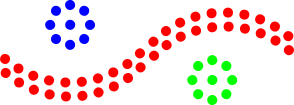
\includegraphics[scale=0.5]{images/dbscan.pdf}
  \caption[Clustering using the DBSCAN algorithm]{Clustering using the DBSCAN algorithm.}
  \label{images:dbscan}
\end{figure}


\section{Document Summarisation}
\label{sec:document-summarisation}

The problem of API summarisation could be linked to the document summarisation one. In fact, it could be viewed as a multi-document summarisation task where, according to \nolink{\citeauthor{Aliguliyev:2010}} \cite{Aliguliyev:2010}, the intention is to create a compressed version of a given collection of documents, that provides useful information to the users. Multi-document text summarisation has been an emerging field throughout the last 15 years. The \textit{Document Understanding Conference}\footnote{\url{http://www-nlpir.nist.gov/projects/duc/index.html}} (DUC), organised since 2001\footnote{DUC is now part of the \textit{Text Analysis Conference} (TAC).}, has been the major forum for comparing summarization systems, while it also included the \textit{multi-document summarization task}, with the purpose of creating fixed-length summaries, for a set of given documents.

When summarising an API, the collection of documents refers to the source code repository that is going to be mined, while the compressed version is in the form of API call sequences, or even better of snippets. A common approach in multi-document summarisation, is to leverage unsupervised techniques, in order to cluster similar sentences. 

For instance, \nolink{\citeauthor{Wang:2008}} make use of semantic analysis, with the purpose of computing similarities between sentences, which they then cluster. This is followed by the retrieval of the most informative sentences from each cluster, which are going to form the summary. Similarly, \nolink{\citeauthor{Boros:2001}} \cite{Boros:2001} use a combination of hierarchical and non-hierarchical clustering techniques, with the aim of partitioning a set of sentences into clusters, with each of them containing sentences covering only a single topic. A more recent approach is the one presented in \cite{Liu:2012}, where \nolink{\citeauthor{Liu:2012}} build a deep learning model, in an attempt to efficiently solve the multi-document summarisation problem.

In addition to the multi-document summarisation problem, we are also going to consider the single-document summarisation task in this dissertation. This task aims to produce a summary of a single document. According to \nolink{\citeauthor{Aliguliyev:2010}} \cite{Aliguliyev:2010}, such a summary could be either \textit{extractive} or \textit{abstractive}. The first one includes these sentences that are considered important, in order for someone to understand the given document, while, according to \nolink{\citeauthor{Aliguliyev:2010}}, the generation of the second one ``usually needs information fusion, sentence compression and reformulation''.


\section{Source Code Summarisation}
\label{sec:source-code-summarisation}

Most of the systems that perform API mining so far present sequences of API method calls, rather than snippets, to the users. Although such sequences may seem interesting, they cannot adequately describe a source code example efficiently. On the other hand, presenting long snippets, such as the entire source code of the client methods that contain the mined sequences, may hinder the understanding of the target API, as these snippets usually contain several non-API relevant statements. This has prompted the authors of most recent publications in API usage mining to try to summarise usage examples \cite{Montandon:2013, Kim:2013}, or even to synthesise them, by combining information of similar snippets \cite{Buse:2012}.

In contrast to text summarisation which is a well-studied field, source code summarisation techniques have only emerged during the last years. These two fields have many similarities, though. \nolink{\citeauthor{Ramanujam:2016}} \cite{Ramanujam:2016} identify three characteristics of a good text summary; \textit{coverage}, \textit{coherence} and \textit{redundancy}. We could claim that both characteristics apply to source code, too. What differentiates, however, the process of text summarisation from that of source code summarisation is that a source code, in contrast to free text, contains semantic as well as structural information. Hence, simple approaches that leverage text summarisation techniques (e.g. $tf/idf$), and that are based on keywords, cannot be efficiently applied to source code as they neglect the semantic context.

Similarly to a single text document summary, the major goal of a code fragment summary is to present the main ideas in the original fragment in less space. There have been interesting studies that try to define what a good source code example, and by extension summary, is. For instance, \nolink{\citeauthor{Nasehi:2012}} \cite{Nasehi:2012} introduce the notion of the \textit{concise code}, which usually contains less than four lines of code, while replacing unnecessary details with placeholders (comments or ellipses). Moreover, \nolink{\citeauthor{Ying:2014}} \cite{Ying:2014} identify common summarisation practices (e.g. shortening identifiers or formatting code for readability) by  conducting user studies.

\nolink{\citeauthor{Ying:2013}} \cite{Ying:2013} introduce a novel way to summarise code fragments, by exploiting ML techniques. Their system trains a classifier, using feature vectors, that contain features which are either syntactic or even related to the query, in order to decide on whether a line of the given source code should be in the summary or not. This is an interesting approach, but a general-purpose one.

Instead, taking into consideration that, in the case of API usage mining, we are mainly interested in statements that contain API-relevant information, \nolink{\citeauthor{Kim:2013}} \cite{Kim:2013} exploit \textit{slicing}\footnote{There have been almost 35 years since \nolink{\citeauthor{Weiser:1981}} \cite{Weiser:1981} defined \textit{program slicing} as a method for isolating only the part of a program that is of interest to the user, based on a slicing criterion. Here, we are primarily interested in \textit{static slicing}, which does not take into consideration the execution of the program.} techniques, to extract only the semantically relevant -to the given API method- lines. In the same direction, \nolink{\citeauthor{Montandon:2013}} \cite{Montandon:2013} devise a summarisation algorithm, which uses \textit{forward} and \textit{backward slicing}\footnote{The purpose of \textit{backward slicing}, is to find these statements that contribute to the -information used in the- defined  criterion, while \textit{forward slicing} identifies the statements that are affected by that.} techniques, with the purpose of excluding the non-API statements. This seems a promising task-specific approach but, as we are going to explain during the analysis of our implementation, this could still result in undesirable redundancy.